\section{Bài 5: FTP}
Cho tập tin FTP$\_$02.cap, đọc tập tin này bằng Wireshark và trả lời các câu hỏi sau.\\
\textbf{a.	FTP sử dụng giao thức nào UDP hay TCP?}\\
FTP sử dụng giao thức TCP (phần đóng khung màu vàng trong hình \ref{fig5a1}).
\begin{figure}[H]
\begin{center}
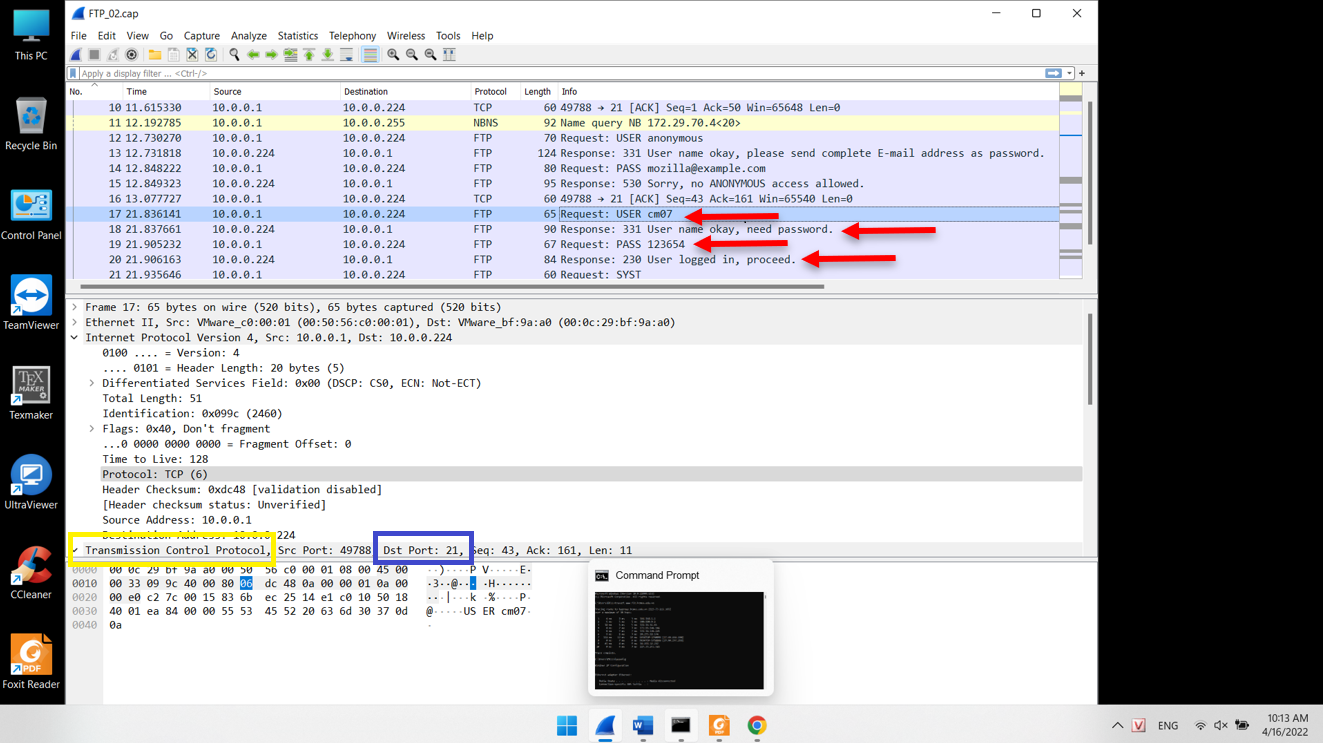
\includegraphics[scale=.8]{../figures/p5/p5_1}
\end{center}
\caption{Giao thức được FTP sử dụng}
\label{fig5a1}
\end{figure}

\textbf{b.	Port mặc định của FTP Server để nhận kết nối là bao nhiêu?}\\
Port mặc định của FTP Server để nhận kết nối là 21 (phần đóng khung màu xanh trong hình \ref{fig5a1}).\\

\textbf{c.	Username và password của người dùng là gì?}\\
Username của người dùng là cm07, password là 123654. Các mũi tên màu đỏ trên hình \ref{fig5a1} thể hiện vị trí thông tin các gói tin tương ứng (các gói tin request, số 17, 19; và các gói tin response tương ứng, số 18, 20). Còn user anonymous ở phía trên không được cho phép kết nối (các gói tin 12 đến 15).

\textbf{d.	Port truyền lệnh của client là bao nhiêu?}\\
Port truyền lệnh của client là port 49788.
\begin{figure}[H]
\begin{center}
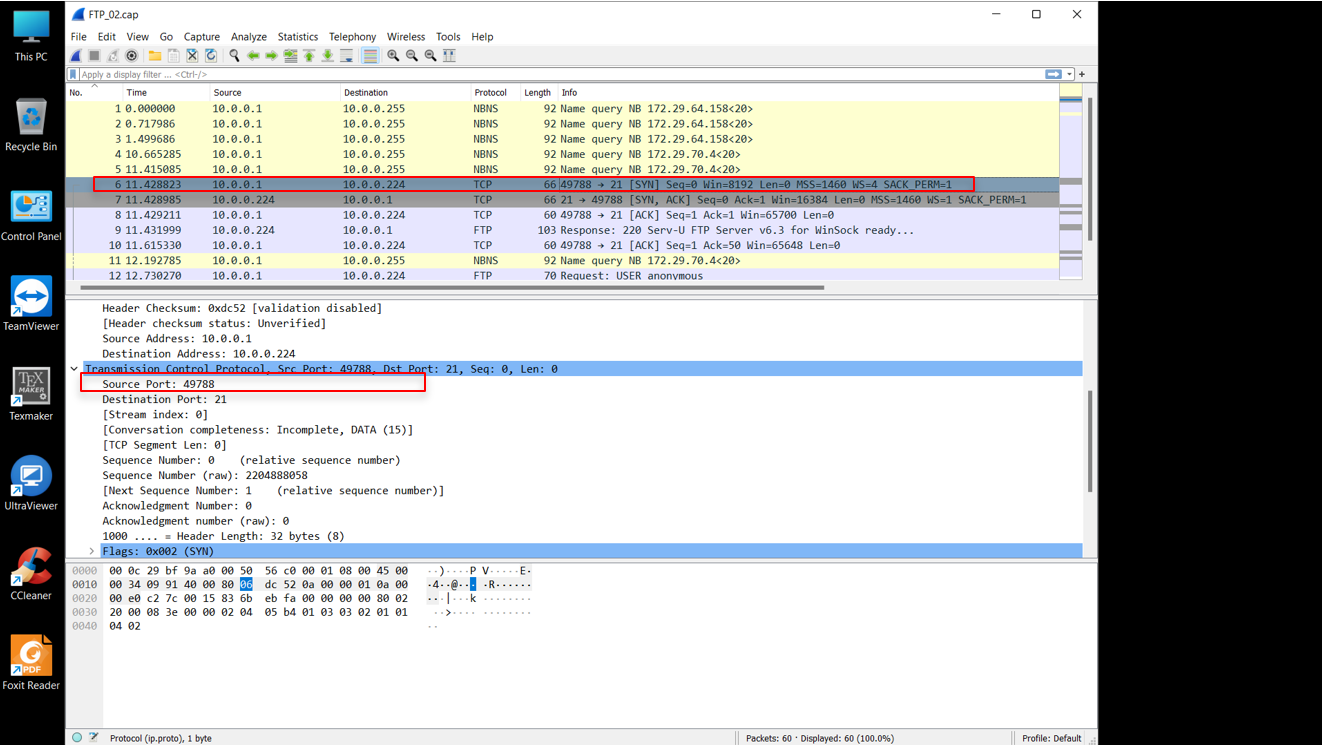
\includegraphics[scale=.8]{../figures/p5/p5_2}
\end{center}
\caption{Port truyền lệnh của client}
%\label{fig5a1}
\end{figure}

\textbf{e.	Client truy xuất lên server theo mode nào: active hay passive?}\\
Client truy xuất lên server theo mode mặc định là active.
Muốn chuyển sang mode passive client cần gửi gói tin request PASV.
\begin{figure}[H]
\begin{center}
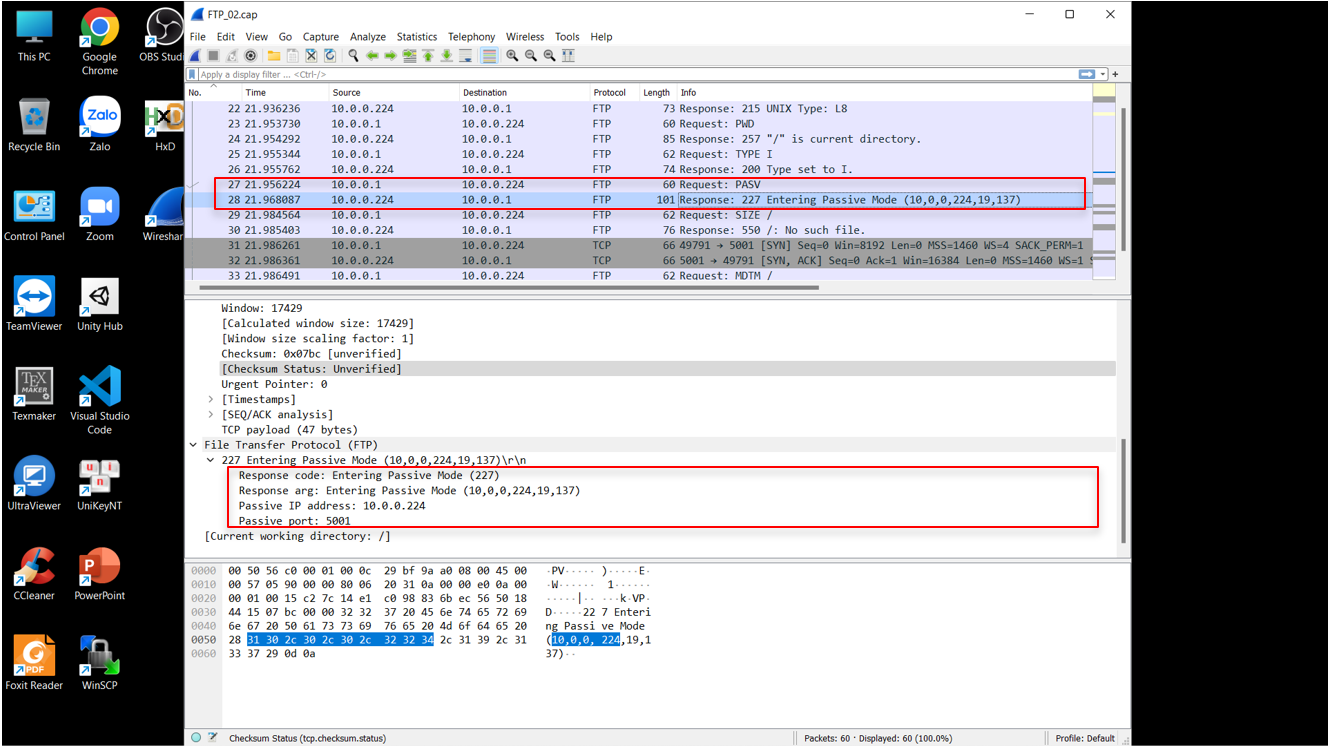
\includegraphics[scale=.8]{../figures/p5/p5_3}
\end{center}
\caption{Thể hiện của gói tin request/response khi muốn vào mode passive}
%\label{fig5a1}
\end{figure}

\textbf{f.	Chỉ ra quá trình bắt tay 3 bước của client và server để tạo kết nối ban đầu khi thực hiện truyền username và password.}
\begin{figure}[H]
\begin{center}
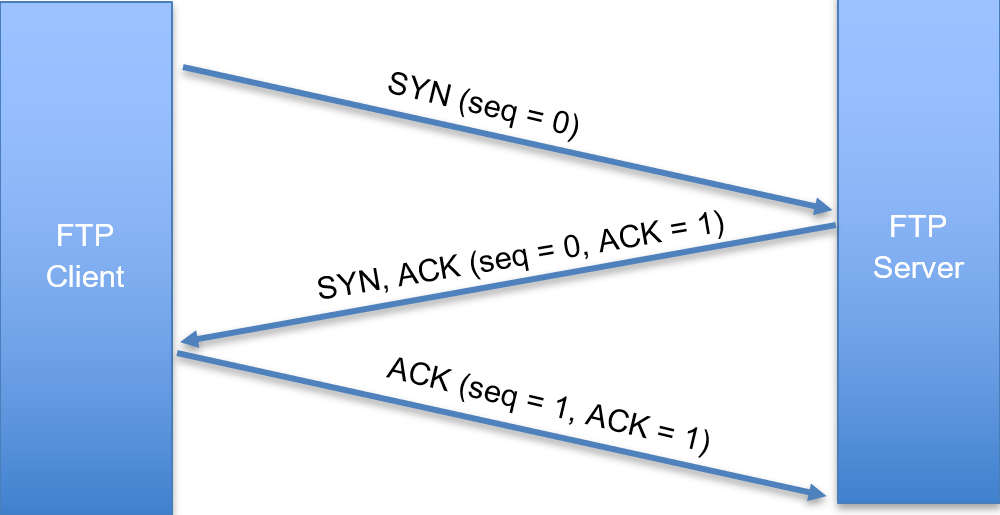
\includegraphics[scale=.6]{../figures/p5/p5_4}
\end{center}
\caption{Quá trình bắt tay 3 bước để tạo kết nối ban đầu}
\end{figure}

\begin{figure}[H]
\begin{center}
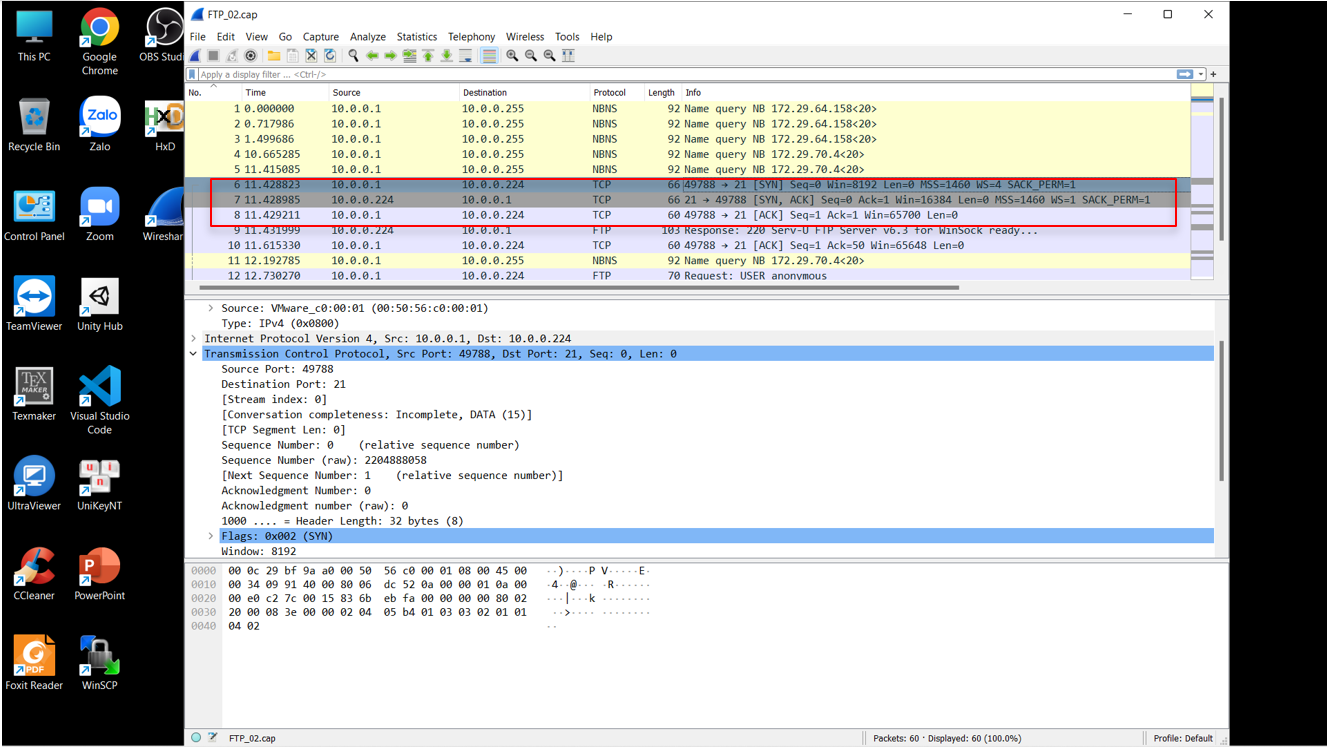
\includegraphics[scale=.8]{../figures/p5/p5_5}
\end{center}
\caption{Quá trình bắt tay 3 bước để tạo kết nối ban đầu}
\end{figure}

\textbf{g.	Chỉ ra quá trình bắt tay 3 bước của client và server để tạo kết nối truyền dữ liệu.}
\begin{figure}[H]
\begin{center}
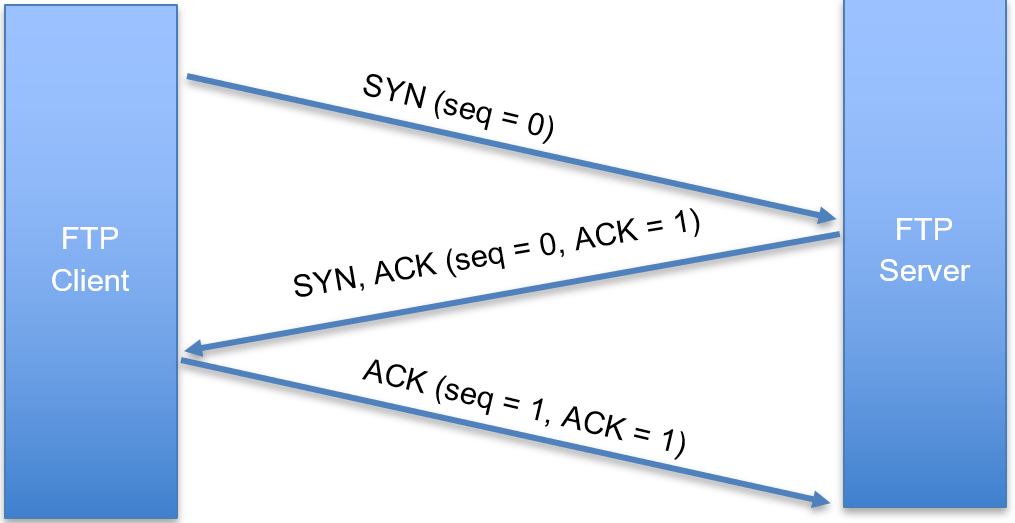
\includegraphics[scale=.6]{../figures/p5/p5_6}
\end{center}
\caption{Quá trình bắt tay 3 bước để tạo kết nối truyền dữ liệu}
\end{figure}

\begin{figure}[H]
\begin{center}
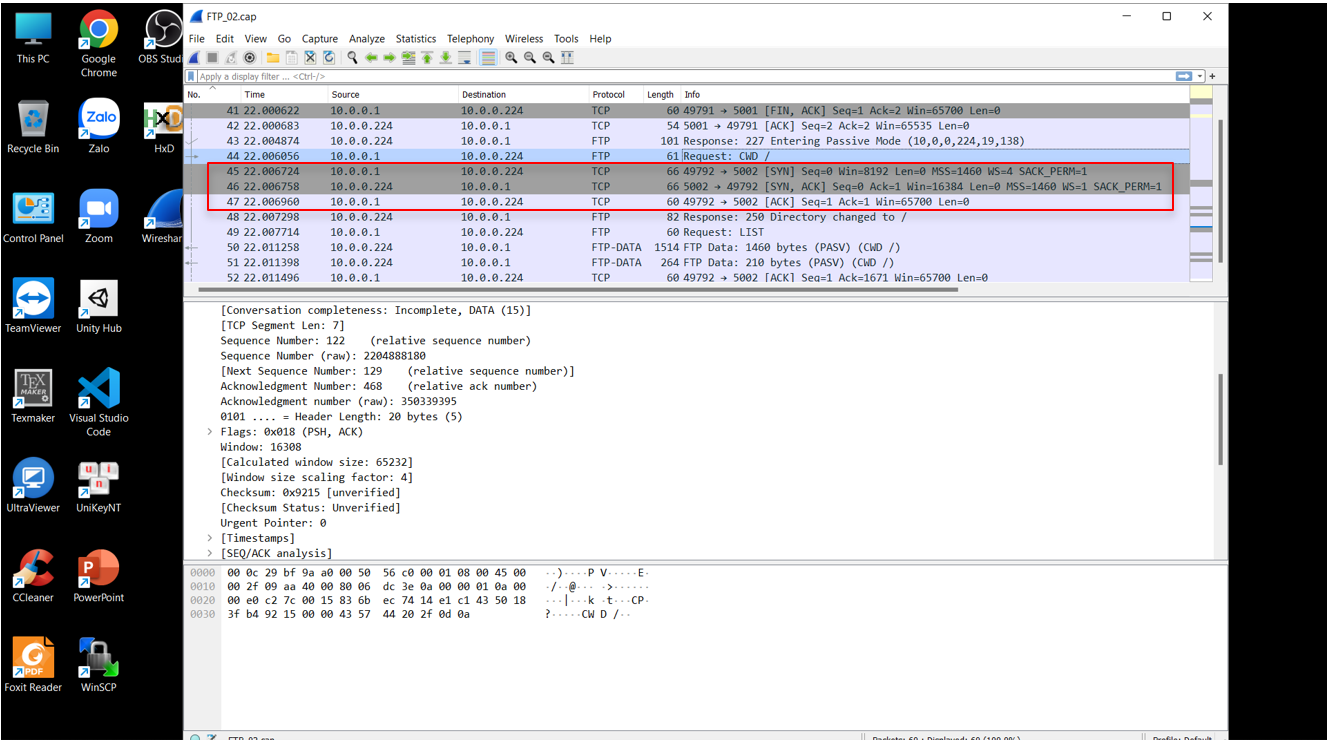
\includegraphics[scale=.8]{../figures/p5/p5_7}
\end{center}
\caption{Quá trình bắt tay 3 bước để tạo kết nối truyền dữ liệu}
\end{figure}

\textbf{h.	Port truyền dữ liệu của FTP server và client là bao nhiêu?}\\
Port truyền dữ liệu của FTP server và client tương ứng là 5002 và 49792. Kết nối này được tạo bởi quá trình bắt tay ba bước ở câu g nêu trên, cụ thể thể hiện ở các gói tin số 45, 46, 47.
Các gói tin liên quan được kẻ khung màu đỏ ở phía trên, khung màu đỏ ở hình \ref{fig5h} (ứng với gói tin số 50, chuyển data từ FTP server sang FTP client) cũng nêu ra port tương ứng.

\begin{figure}[H]
\begin{center}
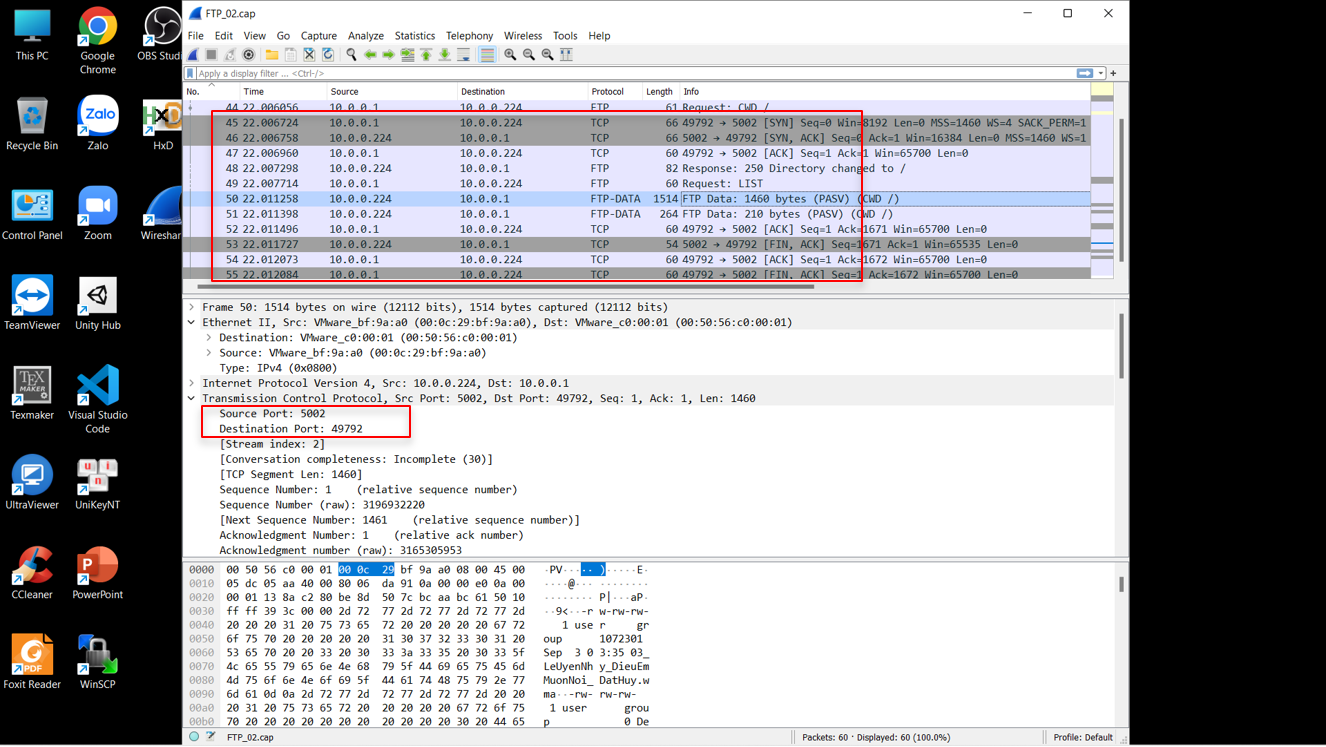
\includegraphics[scale=.8]{../figures/p5/p5_8}
\end{center}
\caption{Port truyền dữ liệu của FTP server và client}
\label{fig5h}
\end{figure}

Trước đó, port truyền dữ liệu của FTP Server và Client tương ứng là 5001 và 49791 (thông tin tương ứng ở các gói tin 31, 32, 34 thể hiện quá trình bắt tay ba bước được nêu ở câu g), và bị ngắt kết nối (các gói tin [FIN,ACK] và [ACK] từ 39 – 42 thể hiện quá trình này).
